\subsection{Protocol}
\label{sec:protocol}

We time the communication module in isolation, with the training loop removed.
The protocol is stated in full because two of its provisions were forced by
defects that produced spurious results first (Section~\ref{sec:pitfalls}).

Timing uses on-device CUDA events with an explicit synchronisation on the
correct device. Any diagnostic that calls \texttt{.item()} is disabled, because
such a call synchronises the device \emph{inside} the timed forward pass. Arms
are timed \textbf{interleaved repetition by repetition} rather than in
sequential per-arm blocks, so that any interference from other tenants lands on
all arms at once and the ratios between them remain paired; on this shared host
the sequential design produced swings above $100\%$ between identical
configurations, which interleaving reduced to typically under $2\%$. We report
$\min$ over samples as the primary statistic, since contention can only add
time, and give median, IQR and inter-run spread for every headline cell in
Appendix~\ref{app:dispersion}. GPU clocks could not be locked --- the account
lacks the privilege --- and we say so rather than implying a controlled clock.
Executed FLOPs are counted with \texttt{torch.utils.flop\_counter} so that
latency is always reported beside the arithmetic actually performed.

Unless stated otherwise: PyTorch 2.11 / CUDA 12.8, \texttt{fp32}, input
embedding width $64$, head width $d{=}16$, batch $256$, $k = 25\%$ of peers,
and an idle device.

\subsection{Three curves}
\label{sec:threecurves}

\begin{table}[t]
\centering
\small
\caption{Forward latency (ms, $\min$ over interleaved samples) of three
implementations of the same function, plus the fused dense baseline. The
gathered path executes fewer FLOPs than dense at every $N$ and is slower at
every $N$. Ratios are gathered relative to each dense baseline.}
\label{tab:headline}
\begin{tabular}{rrrrrrrrr}
\toprule
& & \multicolumn{2}{c}{\textbf{dense}} & \multicolumn{2}{c}{\textbf{top-$k$}} & \multicolumn{2}{c}{\textbf{ratio}} & \textbf{MFLOP} \\
\cmidrule(lr){3-4}\cmidrule(lr){5-6}\cmidrule(lr){7-8}
$N$ & $k$ & fused & unfused & \Mask & \Gath & /unfused & /fused & gath.\,vs dense \\
\midrule
6   & 1   & 0.117 & 0.124 & 0.174 & 0.146 & 1.17 & 1.24 & 11 vs 11 \\
12  & 2   & 0.117 & 0.125 & 0.179 & 0.151 & 1.21 & 1.29 & 22 vs 23 \\
24  & 5   & 0.099 & 0.120 & 0.173 & 0.147 & 1.22 & 1.49 & 47 vs 50 \\
48  & 11  & 0.108 & 0.128 & 0.184 & 0.158 & 1.23 & 1.46 & 105 vs 120 \\
96  & 23  & 0.105 & 0.124 & 0.214 & 0.224 & 1.81 & 2.13 & 257 vs 315 \\
192 & 47  & 0.149 & 0.206 & 0.681 & 0.771 & 3.75 & 5.19 & 703 vs 931 \\
384 & 95  & 0.295 & 1.160 & 3.499 & 3.174 & 2.74 & 10.78 & 2161 vs 3070 \\
512 & 127 & 0.431 & 1.989 & 7.557 & 7.025 & 3.53 & 16.29 & 3553 vs 5167 \\
\bottomrule
\end{tabular}
\end{table}

Table~\ref{tab:headline} is the central result. The gathered implementation
does execute fewer multiply--accumulates than dense --- $3553$ against $5167$
MFLOP at $N{=}512$, a $31\%$ reduction consistent with
Proposition~\ref{prop:ceiling} --- and it is nonetheless $3.53\times$ slower
than unfused dense and $16.29\times$ slower than the fused kernel. Correcting
the implementation matters and is not sufficient: replacing \Mask{} with
\Gath{} improves the ratio from $\approx 1.45\times$ to $\approx
1.23\times$ at small $N$, a real gain that does not reach a crossover.

\paragraph{Robustness.} The ordering is unchanged under
\texttt{torch.compile} and CUDA-graph capture (both within $10\%$ of eager), at
batch $4096$ where the largest cells become FLOP-bound, and in \texttt{bf16}
where all four fused SDPA backends including FlashAttention are reachable --- in
\texttt{bf16} the gap is \emph{wider}, reaching $19.7\times$ the fused kernel at
$N{=}512$. On CPU the ordering also holds, up to $37.9\times$ the fused
baseline, which is the cross-architecture evidence
Section~\ref{sec:roofline} predicts.

\subsection{Is there any $(d, B, N, k)$ where sparsity wins?}
\label{sec:surface}

Reporting isolated favourable cells as anomalies is not a characterisation. We
swept head width $d \in \{32,64,128,256\}$ against batch $\in
\{32,256,4096\}$ and $N \in \{12,48,192,512\}$, and for each cell took the
\emph{best} $k$ for the gather path --- the most favourable case sparsity can
construct for itself.

\begin{table}[t]
\centering
\small
\caption{Best-$k$ gathered latency divided by unfused dense. Values $<1$ would
indicate sparsity winning; none do. ``skip'' marks cells whose activation
memory exceeded the budget (at $d{=}256$, $B{=}4096$, $N{=}512$ the gathered
value tensor alone is $\approx$273\,GiB) and which are recorded as skipped
rather than dropped.}
\label{tab:surface}
\begin{tabular}{rrrrrr}
\toprule
$d$ & batch & $N{=}12$ & $N{=}48$ & $N{=}192$ & $N{=}512$ \\
\midrule
32  & 32   & 1.22 & 1.20 & 1.19 & 2.29 \\
32  & 256  & 1.21 & 1.21 & 1.83 & 2.43 \\
32  & 4096 & 1.35 & 1.98 & 1.48 & 2.36 \\
64  & 32   & 1.22 & 1.22 & 1.22 & 2.35 \\
64  & 256  & 1.23 & 1.22 & 1.76 & 2.46 \\
64  & 4096 & 1.50 & 1.85 & 1.47 & 2.36 \\
128 & 32   & 1.21 & 1.22 & 1.24 & 1.87 \\
128 & 256  & 1.23 & 1.27 & 1.52 & 2.12 \\
128 & 4096 & 1.45 & 1.91 & 1.50 & skip \\
256 & 32   & 1.23 & 1.20 & 1.16 & 1.47 \\
256 & 256  & 1.19 & 1.31 & 1.37 & 1.71 \\
256 & 4096 & 1.28 & 1.61 & 1.45 & skip \\
\bottomrule
\end{tabular}
\end{table}

\begin{figure}[t]
\centering
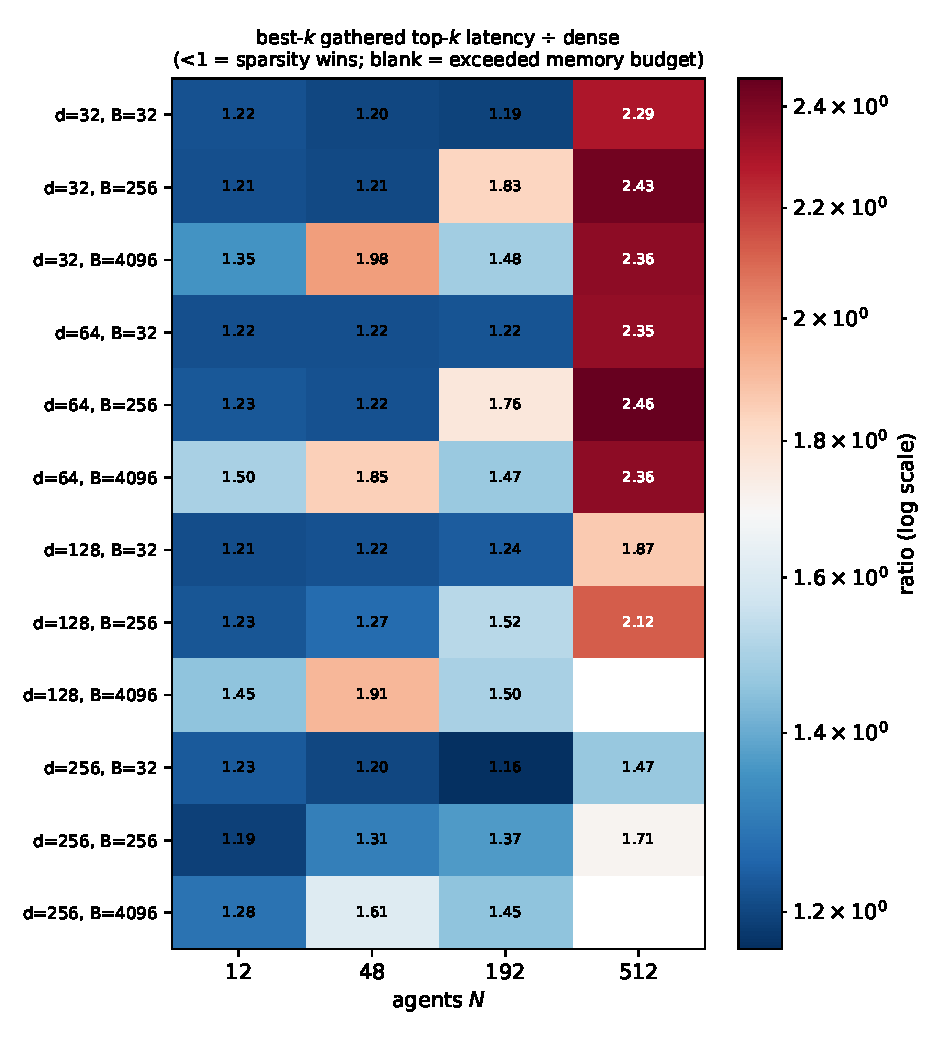
\includegraphics[width=0.62\linewidth]{figures/fig_crossover.pdf}
\caption{The crossover surface of Table~\ref{tab:surface}. Every cell is
$>1$: there is no operating point in the surveyed region at which a
genuinely sparse top-$k$ implementation is faster than dense attention. Blank
cells exceeded the memory budget.}
\label{fig:crossover}
\end{figure}

\textbf{Gathering beats unfused dense in $0$ of $46$ measured cells}, and the
fused baseline in $1$ of $46$ (at $d{=}128$, $B{=}4096$, $N{=}12$, where the
fused kernel's fixed overhead dominates at tiny $N$). The ratio stays within
$1.16$--$2.46\times$ across an eightfold range of head width and a
$128$-fold range of batch. That flatness is itself the finding: the outcome is
structural rather than a consequence of any particular operating point.

\subsection{Where the time goes}
\label{sec:decomp}

Table~\ref{tab:headline} says \emph{that} sparsity loses; the following says
\emph{why}. We time each stage in isolation under the same protocol and form
two quantities: the \emph{saving} the sparse contraction buys
($\texttt{agg\_dense} - \texttt{agg\_sparse}$) and the \emph{overhead}
selection costs
($\texttt{topk} + \texttt{gather} + \texttt{softmax}_k - \texttt{softmax}_N$).

\begin{table}[t]
\centering
\small
\caption{Per-stage latency (ms). The aggregation ``saving'' is \emph{negative}
at every $N$: the sparse contraction is slower than the dense matmul it
replaces, despite performing $\approx4\times$ fewer multiply--accumulates.
Selection overhead is an order of magnitude larger still.}
\label{tab:decomp}
\begin{tabular}{rrrrrrrr}
\toprule
$N$ & $k$ & \texttt{topk} & \texttt{gather} & \texttt{agg\_dense} & \texttt{agg\_sparse} & saving & overhead \\
\midrule
12  & 2   & 0.016 & 0.013 & 0.014 & 0.016 & $-0.003$ & $+0.028$ \\
48  & 11  & 0.037 & 0.012 & 0.015 & 0.021 & $-0.006$ & $+0.047$ \\
96  & 23  & 0.087 & 0.027 & 0.022 & 0.055 & $-0.033$ & $+0.114$ \\
192 & 47  & 0.434 & 0.146 & 0.056 & 0.144 & $-0.088$ & $+0.554$ \\
384 & 95  & 1.427 & 0.554 & 0.174 & 0.495 & $-0.321$ & $+1.824$ \\
512 & 127 & 3.897 & 0.986 & 0.247 & 0.845 & $-0.598$ & $+4.595$ \\
\bottomrule
\end{tabular}
\end{table}

Two facts emerge, and both are stronger than the hypothesis they were meant to
test. First, \textbf{the aggregation saving is negative}: the sparse
$(B\!\cdot\!N,1,k)\times(B\!\cdot\!N,k,d)$ contraction is $3.4\times$
\emph{slower} than the dense $(B,N,N)\times(B,N,d)$ matmul it replaces at
$N{=}512$, because a batched matrix--vector product has far lower arithmetic
intensity than a real GEMM and cannot use the same hardware paths. Second,
\textbf{selection dominates everything}: \texttt{topk} alone costs
$15.8\times$ the entire dense aggregation at $N{=}512$.

The consequence is that the loss is not an engineering defect a better kernel
would remove. It is intrinsic to ranking all $N$ scores --- exactly the
assumption A2 that Proposition~\ref{prop:ceiling} rests on.

\subsection{The learned gate costs $\mathcal{O}(BN^3)$ memory}
\label{sec:memory}

A per-agent learned gate over $k \in \{1,\dots,N-1\}$, implemented in the
natural way, broadcasts a $(1,1,K,N)$ cumulative-keep tensor against
$(B,N,K,1)$ gate probabilities with $K = N-1$, materialising $(B,N,N-1,N)$
before reducing. Activation memory is therefore $\mathcal{O}(BN^3)$ against
dense attention's $\mathcal{O}(BN^2)$ and the fused kernel's
$\mathcal{O}(BNd)$.

We validate the derivation rather than asserting it. Fitting $\text{peak} \sim
N^p$ over $N \ge 48$ with a constant offset removed gives $p = 3.04$ for the
gate, against $1.96$ for dense, $2.02$ for masked, $1.98$ for gathered and
$1.36$ for fused. The sharper check is absolute: at $N{=}384$ the closed form
predicts $97.5\%$ of the measured peak. In practice the gate consumes
$56.5$\,GiB at $N{=}384$ (batch $256$) and exhausts the device at $N{=}512$;
analytically it exhausts a $96$\,GiB card at $N{=}465$, and at batch $4096$ at
$N{=}185$. The arm whose purpose is to reduce cost is the first to run out of
memory.

\subsection{Drift control}
\label{sec:drift}

Because clocks are unlocked and the host is shared, we re-ran the identical
sweep $\approx21$\,h later, twice.

\begin{table}[t]
\centering
\small
\caption{Reproducibility of the headline sweep. Ratios --- the quantity every
claim is stated in --- are far more stable than absolute latency.}
\label{tab:drift}
\begin{tabular}{lrrrr}
\toprule
& \multicolumn{2}{c}{\textbf{latency} $|\Delta|$} & \multicolumn{2}{c}{\textbf{ratio} $|\Delta|$} \\
\cmidrule(lr){2-3}\cmidrule(lr){4-5}
\textbf{Condition} & median & max & median & max \\
\midrule
Idle second device, same model      & 1.9\%  & 6.5\%  & \textbf{1.0\%}  & \textbf{3.2\%} \\
Same device, concurrent training load & 41.3\% & 80.6\% & 25.9\% & 56.4\% \\
\bottomrule
\end{tabular}
\end{table}

On an idle second device the ratios reproduce to within $3.2\%$ at every $N$,
so the measurement is a property of the algorithm and architecture rather than
of one physical card. Under concurrent load agreement degrades substantially,
concentrated at small and moderate $N$ where kernels are launch-bound; the
largest cells move by about $1\%$. We state the consequence plainly:
\textbf{latency must be measured on an unloaded device}, and interleaving plus
minimum-over-samples reduces contention sensitivity without eliminating it.

The direction matters more than the magnitude. \emph{Every} drift moves in the
direction that makes the sparse path look worse, and the smallest
gathered/dense ratio observed anywhere --- across all runs, devices, loads,
precisions and execution modes --- is $1.14\times$. Contention cannot be
concealing a crossover; it can only exaggerate a gap that is already present.
